%%%%%%%%%%%%%%%%%%%%%%%%%%%%%%%%%%%%%%%%%%%%%%%%%%%%%%%%%%%%%%%%%%%%%%%%%%%

\documentclass{standalone}

\usepackage{amsmath}
\usepackage{mathptmx}
\usepackage{pgfplots}
\usetikzlibrary{external}
\tikzexternalize{cricket-run-rsquared}
\pgfplotsset{compat=1.16}

%% IEEE uses Times Roman font, so we'll default to Times.
%% These three commands make up the entire times.sty package.
\renewcommand{\rmdefault}{ptm}
\renewcommand{\ttdefault}{pcr}
\normalfont\selectfont

\begin{document}

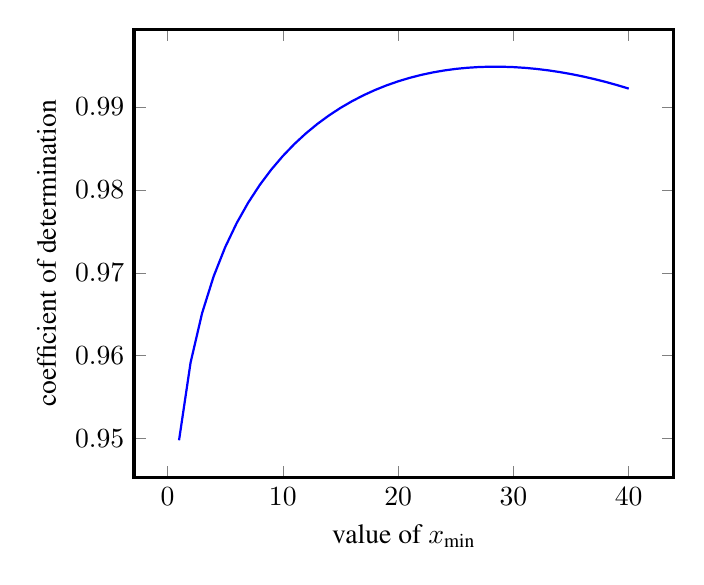
\begin{tikzpicture}
\tikzset{%%
  every mark/.append style={scale=1.0},%%
  scale=1.0%%
}
\pgfplotsset{%%
  every axis/.append style={font=\normalsize}%%
}
%%
\begin{axis}[%%
  axis line style=very thick,%%
  dotStyle/.style={blue,mark=none,thick},%%
  enlargelimits=true,%%
  %% x axis
  xlabel={\normalsize value of $x_{\text{min}}$},%%
  %% y axis
  ylabel={\normalsize coefficient of determination}%%
]
%%
%%
\addplot[dotStyle] coordinates {
  (1, 0.949798)
  (2, 0.959166)
  (3, 0.965137)
  (4, 0.969567)
  (5, 0.973089)
  (6, 0.976000)
  (7, 0.978469)
  (8, 0.980597)
  (9, 0.982454)
  (10, 0.984088)
  (11, 0.985535)
  (12, 0.986820)
  (13, 0.987964)
  (14, 0.988985)
  (15, 0.989895)
  (16, 0.990704)
  (17, 0.991423)
  (18, 0.992058)
  (19, 0.992616)
  (20, 0.993102)
  (21, 0.993521)
  (22, 0.993877)
  (23, 0.994174)
  (24, 0.994415)
  (25, 0.994603)
  (26, 0.994739)
  (27, 0.994827)
  (28, 0.994869)
  (29, 0.994865)
  (30, 0.994818)
  (31, 0.994729)
  (32, 0.994599)
  (33, 0.994431)
  (34, 0.994223)
  (35, 0.993979)
  (36, 0.993698)
  (37, 0.993381)
  (38, 0.993030)
  (39, 0.992644)
  (40, 0.992225)
};
\end{axis}
\end{tikzpicture}

\end{document}
